\chapter{Preliminaries}
\markboth{Preliminaries}{}% To set left/right header
% \localtableofcontents

This chapter first introduce the notion of \emph{closed-loop sensitivity} for quantifying how variations of some models parameters (supposed to be uncertain) affect the evolution of the system in closed-loop, i.e., by also taking into account any controller chosen for executing the task.
Then, we present how the sensitivity metrics can be leveraged to derive \emph{uncertainty tubes} that bounds the system states evolution both in the \emph{input} and \emph{state} spaces.
Finally, we introduce the quadrotor robot and differential drive robot models used in this manuscript.

\section{Closed-loop sensitivity}
\subsection{Definition}

Consider an arbitrary dynamic system with a set of uncertain parameters $\p \in \mathbb{R}^{n_p}$ (i.e. model parameters that are difficult to evaluate or likely to vary during a motion).
The system dynamics can be described using the following set of ordinary differential equations (\myglsentry{odes}):
\begin{equation}\label{eq:dyna}
    \dot{\q}=\f(\q,\,\u,\,\p), \quad \q(t_0)=\q_{0},
\end{equation}
where $\q\in \mathbb{R}^{n_{q}}$ is the system state vector and $\u\in \mathbb{R}^{n_{u}}$ the control input vector.
Also, assume the presence of a controller $\boldmu$ of any form to track a \emph{desired trajectory} $\q_d(t)$ such that:
\begin{equation}\label{eq:ctrl}
     \left \{
     \begin{array}{l l}
          \dot{\bxi} = \g(\bxi,\,\q,\,\q_d,\,\p_n,\,\k_c,\,t), \quad \bxi(t_0)=\bxi_{0}, \\
          \u=\boldmu(\bxi,\,\q,\,\q_d,\,\p_n,\,\k_c,\,t), 
   \end{array} 
   \right .
\end{equation}
where $\bxi\in \mathbb{R}^{n_{\xi}}$ are the internal states of the controller (e.g., an integral action), $\k_{c}\in \mathbb{R}^{n_{k}}$ the controller gains, and $\p_{n}\in{\mathbb{R}^{n_{p}}}$ is the vector of "nominal" system parameters used in the control loop, i.e. the estimated nominal values of $\p$.

In line with the previous definitions, the following sections of this thesis will then differentiate between three types of state vectors of key importance:
\begin{enumerate}
  \item $\q_d$: The \emph{desired} system state vector which refers to the desired values of the controllable system states. This state vector is typically the output of a motion planner. Note that the dimension of this vector may differ from that of the real system because the vector represents a simplified or abstracted model, which might omit certain physical aspects or constraints that are present in the actual system, particularly in the case of under-actuated systems, where not all degrees of freedom are controlled.
  \item $\q_n$: The \emph{nominal} system state vector which represents the real state values of the system during the execution under nominal parameters (i.e. when the uncertain system parameters $\p$ perfectly match the parameter values used in the control loop $\p_n$). A distinction is made between the nominal states and the desired states, as they are generally not equal due to factors such as controller settings, system dynamics, or transient behavior.
  \item $\q$: The \emph{uncertain} system state vector which refers to the real state values of the system during the execution, influenced by a set of uncertain parameters.
\end{enumerate}
Note that the same notations apply to the control input vector as well (e.g., $\u_n$ represents the "nominal" control input values, i.e., when $\p=\p_n$).

It is possible to quantify how the presence of uncertain parameters (i.e. when the real system parameters $\p$ deviate from the nominal value $\p_n$ used in the control loop) affects the evolution of $\q(t)$ and $\u(t)$ according to the following matrices:
\begin{equation}\label{eq:sensi}
  \bPi(t)=\left.\frac{\partial \q(t)}{\partial \p}\right|_{\p=\p_n} \quad\quad \bTheta(t)=\left.\frac{\partial \u(t)}{\partial \p}\right|_{\p=\p_n}
\end{equation}
where $\bPi(t)\in \mathbb{R}^{n_q \times n_p}$ and $\bTheta(t)\in \mathbb{R}^{n_u \times n_p}$ are respectively defined in~\cite{cPi,cTh} as the \emph{state-sensitivity matrix} and the \emph{input-sensitivity matrix}.
A closed-form expression for Equation~(\ref{eq:sensi}) is, in general, not available. 
However, as shown in~\cite{cPi,cTh}, their evolution in time can be computed by differentiating Equation~(\ref{eq:sensi}) and introducing the \emph{internal state sensitivity} matrix $\bPixi(t)\in \mathbb{R}^{n_{\xi} \times n_p}$ s.t.:
\begin{equation}\label{eq:dyna_sensi}
  \left \{
  \begin{array}{l l l}
       \dot{\bPi}(t) = \boldsymbol{\frac{\partial{f}}{\partial{q}}}\bPi+ \boldsymbol{\frac{\partial{f}}{\partial{u}}}\bTheta+ \boldsymbol{\frac{\partial{f}}{\partial{p}}}, \quad \bPi(t_0)=\bPi_0, \\
       \dot{\bPi}_{\xi}(t) = \boldsymbol{\frac{\partial{g}}{\partial{q}}}\bPi+ \boldsymbol{\frac{\partial{g}}{\partial{\xi}}}\bPi_{\xi}, \quad \bPi_{\xi}(t_0)=\bPi_{\xi0}, \\
       \bTheta(t) = \boldsymbol{\frac{\partial{h}}{\partial{q}}}\bPi+ \boldsymbol{\frac{\partial{h}}{\partial{\xi}}}\bPi_{\xi} 
  \end{array}
  \right .
\end{equation}

Now that the sensitivity matrices are defined, one can compute and minimize a chosen norm of $\bPi(t)$ and $\bTheta(t)$ w.r.t. the desired trajectory $\q_d(t)$. 
This optimization generates a desired trajectory with minimal sensitivity, ensuring that the closed-loop evolution of $\q(t)$/$\u(t)$ closely follows its evolution in the nominal case $\q_n(t)$/$\u_n(t)$.

\subsection{Tube computation}

An additional important property of these matrices is that they can be leveraged to derive \emph{uncertainty tubes}, that bounds the closed-loop system trajectory $\q(t)$/$\u(t)$ around its nominal trajectory $\q_n(t)$/$\u_n(t)$ as shown in~\cite{cTube}.
In the following, we remind how to establish bounds around the nominal state trajectory $\q_n(t)$ by focusing solely on the state-sensitivity matrix $\bPi(t)$ for clarity. 
However, it is important to note that this same procedure can also be applied to compute bounds around the nominal input trajectory $\u_n(t)$ by leveraging the input-sensitivity matrix $\bTheta(t)$.

The uncertainty tube for each component of the state is characterized by a \emph{radius} which bounds the state component evolution from its nominal value over time, i.e. for the $i$-th component of the state ($q_i(t)$) the tube radius $r_{q,i}(t)$ is defined as:
\begin{equation}\label{eq:bounds_q}
   r_{q,i}(t) \geq q_i(t) - q_{n,i}(t).
\end{equation}
Let $\Delta\q(t) = \q(t) - \q_n(t)$, representing the deviation of the perturbed trajectory from the nominal one, which we seek to bound.
Assume that for each uncertain parameter $p_{i \in [1, n_p]}$ in $\p$, we have a bounded deviation $\delta p_i \in \mathbb{R}$ s.t. $\forall i \in [1, n_p] ,p_i \in [p_{n_i}-\delta p_i, p_{n_i}+\delta p_i]$.
Without loss of generality, assuming small parameters variations (i.e. small $\delta p$) s.t. $\Delta\q \approx \bPi(t) \Delta\p$, it is possible to obtain an ellipsoid in the state space centered at $\q_n$ as demonstrated in~\cite{cTube}.
The ellipsoid is defined as follows:
\begin{equation}\label{eq:ellipsoid}
  \Delta\q^T (\bPi \bW \bPi^T)^\dag \Delta\q \leq 1,
\end{equation}
where $\bW$ is the following diagonal weight matrix
\begin{equation*}
  \bW = \begin{bmatrix}
    \delta p_1^2 & 0 & \cdots & 0 \\
    0 & \delta p_2^2 & \cdots & 0 \\
    \vdots & \vdots & \ddots & \vdots \\
    0 & 0 & \cdots & \delta p_{n_p}^2
    \end{bmatrix} \in \mathbb{R}^{n_p \times n_p}.
\end{equation*}
Letting the kernel of this ellipsoid defined as $\boldsymbol{K_{\Pi}}(t) = \boldsymbol{\Pi}(t)\boldsymbol{W}\boldsymbol{\Pi}(t)^T$, ~\cite{cTube} as shown how to project the ellipsoid along the $i$-th basis vector component $\boldsymbol{n}_i$ s.t.


\section{Models considered in this thesis}

\subsection{Quadrotor robot application} \label{sec:quad_model}

\begin{figure} [t]
    \centering
    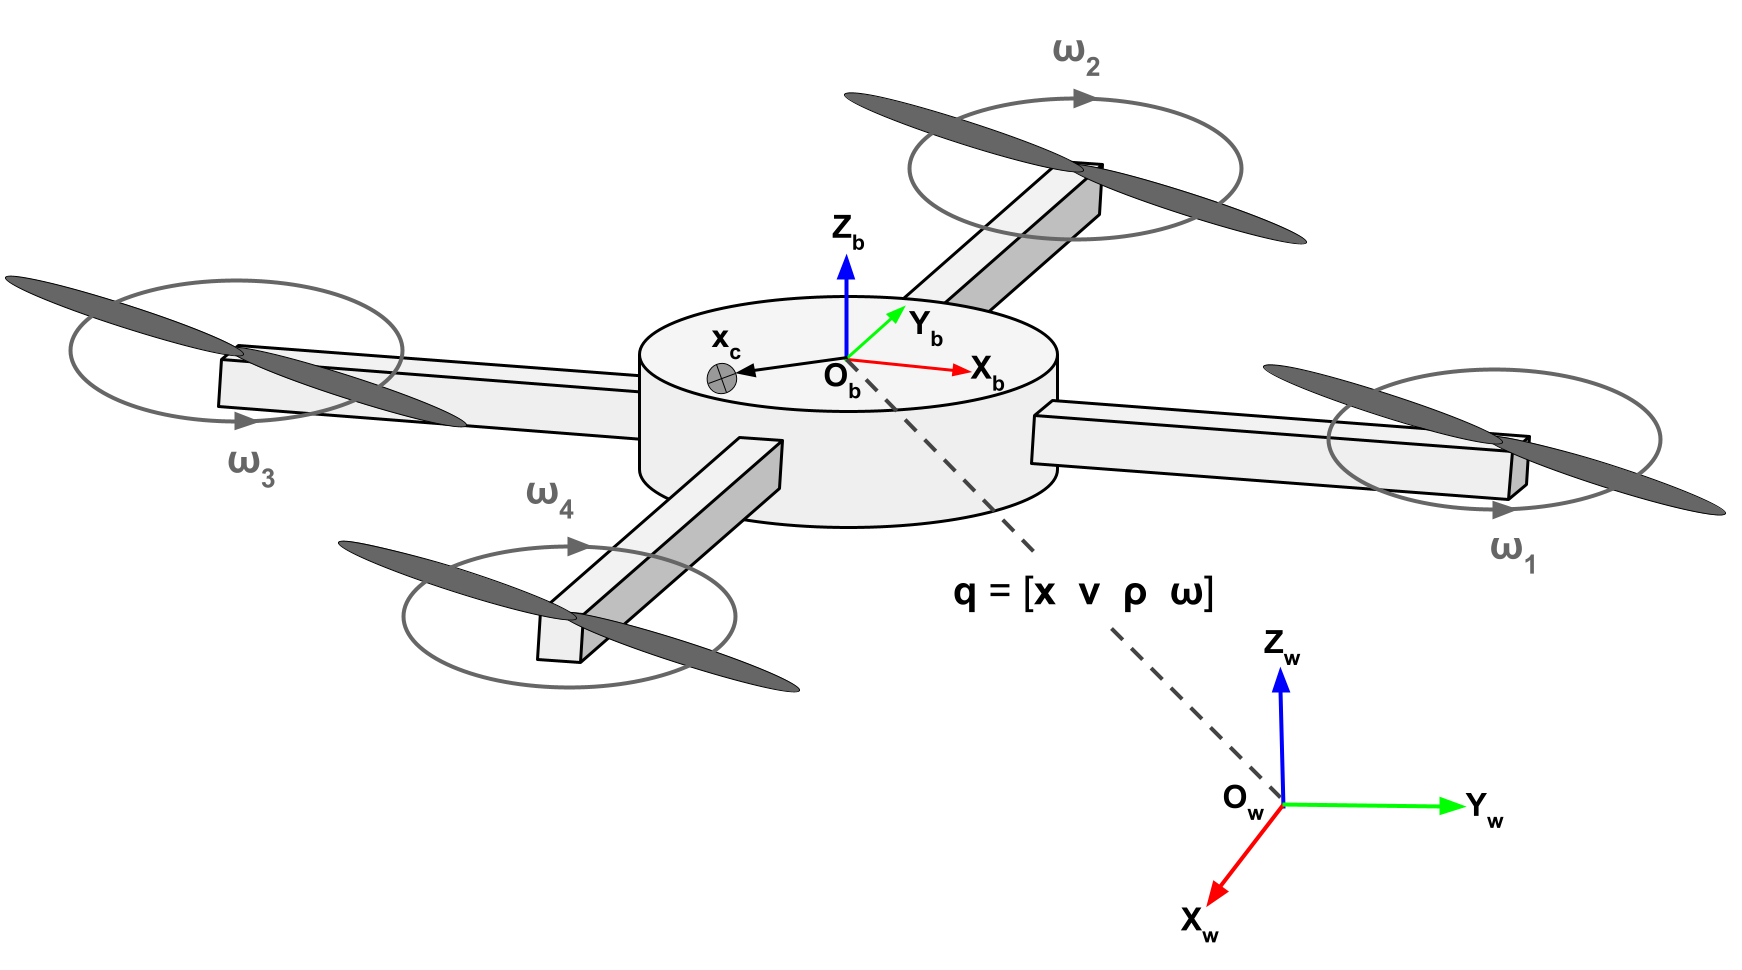
\includegraphics[width=0.8\linewidth]{figures/models/drone.png} 
    \caption{Quadrotor robot representation with a shift in the center of mass.}%
    \label{fig:quad}%
\end{figure}

Let the ENU (East North Up) world frame be defined as $F_W \allowbreak = \allowbreak \{O_W, \allowbreak X_W, \allowbreak Y_W, \allowbreak Z_W\}$ and $F_B = \allowbreak\{O_B, \allowbreak X_B, \allowbreak Y_B, \allowbreak Z_B\}$ be the quadrotor body frame attached to its geometric center ($O_B$).
The state of the quadrotor is defined as $\boldsymbol{q} = [\boldsymbol{x}  \, \boldsymbol{v} \, \boldsymbol{\rho} \, \boldsymbol{\omega}]$ where $\boldsymbol{x} = [x \, y \,z] \in \mathbb{R}^{3}$ and $\boldsymbol{v} = [v_x \, v_y \,v_z] \in \mathbb{R}^{3}$ are respectively the position and velocity vector of $O_B$ expressed in $F_W$. The body orientation w.r.t. $F_W$ is represented by the unitary quaternion  $\boldsymbol{\rho}$ and its angular velocity as $\boldsymbol{\omega} = [\omega_x \, \omega_y \, \omega_z] \in \mathbb{R}^{3}$. 
Finally, let $\boldsymbol{R(\rho)}$ be the rotation matrix associated to $\boldsymbol{\rho}$.

We consider that the center of mass is displaced from the robot's geometric center of an offset $\boldsymbol{x_{c}} = [x_{cx}, x_{cy}, x_{cz}]$ expressed in $F_B$. 
Under this consideration, the total force ($\boldsymbol{f_{tot}}$) and torque ($\boldsymbol{\tau_{tot}}$) acting on the quadrotor can be expressed in $F_B$ s.t. 
\[
    \begin{array}{@{}l@{}l@{}}
        \boldsymbol{f_{tot}} &= f Z_W - mg\boldsymbol{R(\rho)}^TZ_W-m[\boldsymbol{\omega}]_{\times}[\boldsymbol{\omega}]_{\times}\boldsymbol{x_c} 
          
          \\
      
       \boldsymbol{\tau_{tot}} &= \boldsymbol{\tau}-mg[\boldsymbol{x_c}]_{\times}\boldsymbol{R(\rho)}^{T}Z_W - [\boldsymbol{\omega}]_{\times}(\boldsymbol{J}-[\boldsymbol{x_c}]_{\times}[\boldsymbol{x_c}]_{\times})\boldsymbol{\omega}
  \end{array}
\]
where $f$ and $\boldsymbol{\tau}$ are the propeller total thrust and torques, $m$ is the mass and $\boldsymbol{J}$ is the inertia matrix of the system. 
By considering the spatial inertia matrix
\[
\boldsymbol{S} =   \left( {\begin{array}{cc}
    m\boldsymbol{I_3} & -m[\boldsymbol{x_c}]_{\times} \\
    m[\boldsymbol{x_c}]_{\times} & \boldsymbol{J}-m[\boldsymbol{x_c}]_{\times}[\boldsymbol{x_c}]_{\times} \\
  \end{array} } \right)
\]
one finally gets the body frame linear acceleration $\boldsymbol{\alpha}$ and angular acceleration $\boldsymbol{\eta}$
as: 
$
\left( 
    \boldsymbol{\alpha}^T \; \boldsymbol{\eta}^T \right)^T 
  =
  \boldsymbol{S}^{-1}
  \left( \boldsymbol{f_{tot}}^T \;
    \boldsymbol{\tau_{tot}}^T \right)^T. 
$
The dynamic model is then defined as follows:
\begin{equation}\label{eq:dynamic}
    \Dot{\q}
    =
     \left \{
     \begin{array}{l l}
           \dot{\boldsymbol{x}} = \boldsymbol{v} \\
           
           \dot{\boldsymbol{v}}= \boldsymbol{\alpha} \\

           \dot{\boldsymbol{\rho}}=\frac{1}{2}
               \boldsymbol{\rho} \otimes \boldsymbol{\omega} \\
           
           \dot{\boldsymbol{\omega}}=\boldsymbol{\eta}
   \end{array}
   \right .
\end{equation}

As tracking controller, we consider the so-called Lee (or geometric) controller~\cite{cLee} where the control inputs are the squared rotor speeds $\u = [\omega_{1}^2 \, \omega_{2}^2 \, \omega_{3}^2 \, \omega_{4}^2]^T$ that are related to $f$ and $\boldsymbol{\tau}$ by mean of a standard allocation matrix.

The uncertain parameters vector is defined as
$\p$ = $[m, \, x_{cx}, \, x_{cy}, \, J_{x}, \, J_{y}, \,J_{z}]^T \in \mathbb{R}^{6}$, which represents parameters that are difficult to evaluate or likely to vary during execution. 
We chose as nominal parameters $\p_{c}$ = $[1.113, 0.0, 0.0, 0.015, 0.015, 0.007]^T$ and their associated uncertainty range $\delta\p = [7\%, 3cm, 3cm, 10\%, 10\%, 10\%]^T$, which represents the percentage variation of the parameters w.r.t. their associated nominal value, except for $x_{cx}$ and $x_{cy}$ whose nominal values are zeros.

\subsection{Differential drive robot application}

\todomarker{}